\documentclass[11pt,spanish]{beamer}
\usepackage{mathpazo}
\usepackage{tgheros}
\renewcommand{\familydefault}{\sfdefault}
\usepackage[T1]{fontenc}
\usepackage[utf8]{inputenc}
\usepackage{babel}
\usepackage{amsmath}
\usepackage{amssymb}
\usepackage{array}
\usepackage{tikz}
\usetikzlibrary{arrows.meta,calc,positioning,shapes.geometric}

\definecolor{Guinda}{rgb}{0.49, 0.05, 0.12}
\definecolor{Rojo}{rgb}{0.8, 0, 0}
\definecolor{indiagreen}{rgb}{0.07, 0.53, 0.03}
\definecolor{anti-flashwhite}{rgb}{0.95, 0.95, 0.96}
\definecolor{pastelblue}{rgb}{0.78, 0.87, 0.96}
\definecolor{pastelgreen}{rgb}{0.82, 0.92, 0.78}
\definecolor{pastelpeach}{rgb}{0.98, 0.84, 0.72}
\definecolor{pastelrose}{rgb}{0.96, 0.78, 0.84}
\definecolor{pastelviolet}{rgb}{0.86, 0.80, 0.96}
\definecolor{pastelyellow}{rgb}{0.98, 0.93, 0.70}

\usecolortheme[named=indiagreen]{structure}
\usetheme{Boadilla}
\usefonttheme{structurebold}
\setbeamertemplate{itemize items}[default]
\setbeamertemplate{enumerate items}[default]
\setbeamertemplate{navigation symbols}{}
\setbeamercolor{block title}{fg=white,bg=indiagreen!85!black}
\setbeamercolor{block body}{fg=black,bg=pastelgreen!45!white}

\addto\shorthandsspanish{\spanishdeactivate{~<>.}}
\newcommand{\term}[1]{\textbf{\textcolor{indiagreen!80!black}{#1}}}
\newcommand{\actividad}[1]{\textbf{\textcolor{Rojo}{#1}}}
\newcolumntype{L}[1]{>{\raggedright\arraybackslash}p{#1}}

\hyphenpenalty=9000
\exhyphenpenalty=9000
\emergencystretch=2em

\tikzset{
  idea/.style={
    rounded corners=3pt,
    draw=indiagreen!70!black,
    fill=pastelgreen,
    align=center,
    inner sep=7pt,
    font=\small
  },
  bloque/.style={
    rounded corners=3pt,
    draw=black!35,
    fill=pastelblue,
    align=center,
    text width=2.8cm,
    minimum height=1.05cm,
    inner sep=5pt,
    font=\small
  },
  mini/.style={
    rounded corners=3pt,
    draw=black!35,
    fill=anti-flashwhite,
    align=center,
    text width=2.35cm,
    minimum height=.85cm,
    inner sep=4pt,
    font=\scriptsize
  },
  paso/.style={
    rounded corners=3pt,
    draw=indiagreen!70!black,
    fill=pastelgreen,
    align=center,
    text width=2.05cm,
    minimum height=.95cm,
    inner sep=4pt,
    font=\scriptsize
  },
  arrow/.style={
    -{Stealth[length=2.5mm]},
    thick,
    indiagreen!80!black
  }
}

\title[PDS]{\textbf{Panorama de la programación de sistemas}}
\subtitle{Repaso de la Nota 01 y trabajo con el Cuadernillo 01}
\author[Soto Romero y Reyes Cabello]{Manuel Soto Romero \and Araceli Liliana Reyes Cabello}
\institute[UACM]{Colegio de Ciencia y Tecnología, UACM}
\date{Semestre 2026-2}

\begin{document}

\begin{frame}
\titlepage
\end{frame}

\ifkahoot
\begin{frame}{Iniciamos con \textsc{Kahoot}}
\vfill

\begin{center}
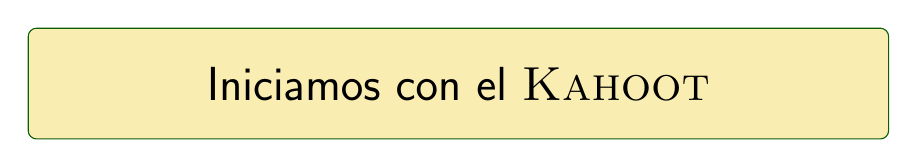
\begin{tikzpicture}
\node[
  idea,
  fill=pastelyellow,
  text width=.82\textwidth,
  inner sep=14pt,
  font=\LARGE
]
{Iniciamos con el \textsc{Kahoot}};
\end{tikzpicture}

\bigskip

\large Los tres mejores lugares reciben una participación.
\end{center}

\vfill
\end{frame}
\fi

\begin{frame}{Pregunta para iniciar el repaso}
\vfill

\begin{center}
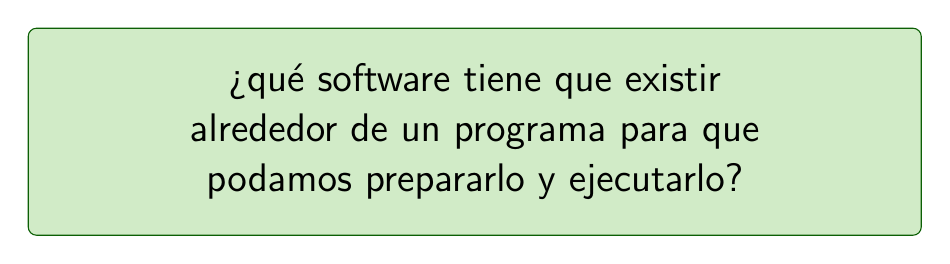
\begin{tikzpicture}
\node[
  idea,
  fill=pastelgreen,
  text width=.86\textwidth,
  inner sep=13pt,
  font=\Large
]
{¿qué software tiene que existir alrededor de un programa para que podamos prepararlo y ejecutarlo?};
\end{tikzpicture}
\end{center}

\bigskip

\begin{block}{Punto de partida}
Un programa no se ejecuta aislado: utiliza herramientas y servicios con responsabilidades distintas.
\end{block}

\vfill
\end{frame}

\begin{frame}{Software de sistemas y programación de sistemas}
\vfill

\begin{columns}[T,onlytextwidth]
\begin{column}{.48\textwidth}
\begin{block}{Software de sistemas}
\small
Conjunto de programas que apoya la operación y el uso de una computadora, y proporciona servicios para preparar, traducir, ejecutar o controlar otros programas.
\end{block}
\end{column}
\begin{column}{.48\textwidth}
\begin{block}{Programación de sistemas}
\small
Área que se ocupa del diseño y la implementación de ese software y de los mecanismos que conectan programas, herramientas y recursos de cómputo.
\end{block}
\end{column}
\end{columns}

\bigskip

\begin{center}
\term{El foco está en la infraestructura que permite usar y ejecutar programas.}
\end{center}

\vfill
\end{frame}

\begin{frame}{Programación de aplicaciones y de sistemas}
\vfill

\begin{center}
\small
\renewcommand{\arraystretch}{1.25}
\begin{tabular}{|L{.42\textwidth}|L{.42\textwidth}|}
\hline
\textbf{Programación de aplicaciones} & \textbf{Programación de sistemas} \tabularnewline
\hline
Se concentra en un problema de una persona u organización. & Se concentra en la infraestructura de software que permite preparar y ejecutar programas. \tabularnewline
\hline
Su producto realiza una tarea concreta. & Su producto ofrece servicios a otros programas o administra recursos. \tabularnewline
\hline
Pregunta: ¿qué resultado necesita la persona usuaria? & Pregunta: ¿qué mecanismos necesita el programa para ejecutarse? \tabularnewline
\hline
\end{tabular}
\end{center}

\bigskip

\begin{center}
\small La diferencia está en el foco principal, no en una jerarquía entre ambas.
\end{center}

\vfill
\end{frame}

\begin{frame}{Características de la programación de sistemas}
\vfill

\begin{center}
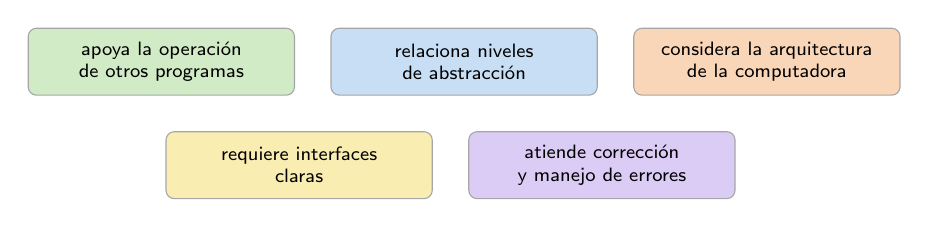
\begin{tikzpicture}[node distance=.45cm]
\node[mini, fill=pastelgreen, text width=3.1cm] (a) {apoya la operación\\de otros programas};
\node[mini, fill=pastelblue, right=of a, text width=3.1cm] (b) {relaciona niveles\\de abstracción};
\node[mini, fill=pastelpeach, right=of b, text width=3.1cm] (c) {considera la arquitectura\\de la computadora};
\node[mini, fill=pastelyellow, below=of a, xshift=1.75cm, text width=3.1cm] (d) {requiere interfaces\\claras};
\node[mini, fill=pastelviolet, right=of d, text width=3.1cm] (e) {atiende corrección\\y manejo de errores};
\end{tikzpicture}
\end{center}

\bigskip

\begin{block}{Recordemos}
Una herramienta recibe una representación, realiza una tarea y produce otra representación o prepara la ejecución.
\end{block}

\vfill
\end{frame}

\begin{frame}{Trabajo con el cuadernillo}
\vfill

\begin{center}
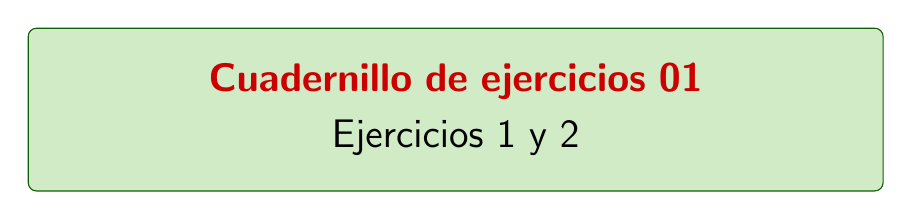
\begin{tikzpicture}
\node[
  idea,
  fill=pastelgreen,
  text width=.82\textwidth,
  inner sep=13pt,
  font=\Large
]
{\actividad{Cuadernillo de ejercicios 01}\\[2pt]
Ejercicios 1 y 2};
\end{tikzpicture}
\end{center}

\bigskip

\begin{itemize}
\item \textbf{Esencial --- Ejercicio 1:} completar las ideas centrales.
\item \textbf{Extensión --- Ejercicio 2:} distinguir aplicaciones y software de sistemas.
\end{itemize}

\vfill
\end{frame}

\begin{frame}{Principales áreas y herramientas}
\vfill

\begin{center}
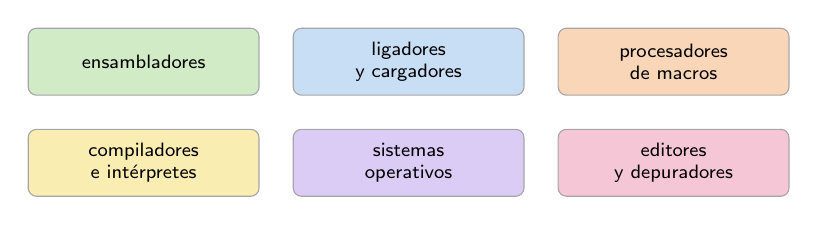
\begin{tikzpicture}[node distance=.42cm]
\node[mini, fill=pastelgreen, text width=2.65cm] (a) {ensambladores};
\node[mini, fill=pastelblue, right=of a, text width=2.65cm] (b) {ligadores\\y cargadores};
\node[mini, fill=pastelpeach, right=of b, text width=2.65cm] (c) {procesadores\\de macros};
\node[mini, fill=pastelyellow, below=of a, text width=2.65cm] (d) {compiladores\\e intérpretes};
\node[mini, fill=pastelviolet, right=of d, text width=2.65cm] (e) {sistemas\\operativos};
\node[mini, fill=pastelrose, right=of e, text width=2.65cm] (f) {editores\\y depuradores};
\end{tikzpicture}
\end{center}

\bigskip

\begin{center}
\small Las áreas se distinguen por su responsabilidad general y pueden colaborar en una misma cadena.
\end{center}

\vfill
\end{frame}

\begin{frame}{¿Qué responsabilidad tiene cada herramienta?}
\vfill

\begin{center}
\scriptsize
\renewcommand{\arraystretch}{1.12}
\begin{tabular}{|L{.26\textwidth}|L{.59\textwidth}|}
\hline
\textbf{Herramienta} & \textbf{Responsabilidad general} \tabularnewline
\hline
Ensamblador & Traduce lenguaje ensamblador a código objeto o de máquina. \tabularnewline
\hline
Ligador & Reúne código objeto y bibliotecas para formar un ejecutable. \tabularnewline
\hline
Cargador & Coloca el programa en memoria y lo prepara para su ejecución. \tabularnewline
\hline
Procesador de macros & Reconoce macros y las expande en secuencias del lenguaje. \tabularnewline
\hline
Sistema operativo & Administra recursos y proporciona servicios para ejecutar programas. \tabularnewline
\hline
Editor / depurador & Apoya la creación del programa / ayuda a observar su ejecución y localizar errores. \tabularnewline
\hline
\end{tabular}
\end{center}

\vfill
\end{frame}

\begin{frame}{Del código fuente a la memoria}
\vfill

\begin{center}
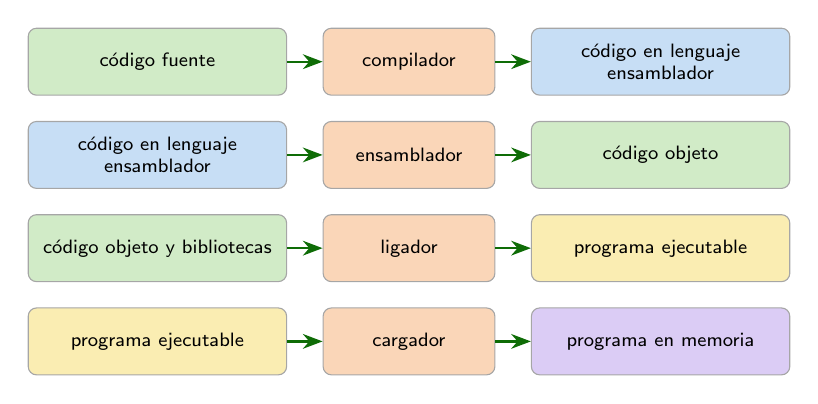
\begin{tikzpicture}[node distance=.32cm and .45cm]
\node[mini, fill=pastelgreen, text width=3cm] (a1) {código fuente};
\node[mini, fill=pastelpeach, right=of a1, text width=1.9cm] (t1) {compilador};
\node[mini, fill=pastelblue, right=of t1, text width=3cm] (b1) {código en lenguaje ensamblador};

\node[mini, fill=pastelblue, below=of a1, text width=3cm] (a2) {código en lenguaje ensamblador};
\node[mini, fill=pastelpeach, right=of a2, text width=1.9cm] (t2) {ensamblador};
\node[mini, fill=pastelgreen, right=of t2, text width=3cm] (b2) {código objeto};

\node[mini, fill=pastelgreen, below=of a2, text width=3cm] (a3) {código objeto y bibliotecas};
\node[mini, fill=pastelpeach, right=of a3, text width=1.9cm] (t3) {ligador};
\node[mini, fill=pastelyellow, right=of t3, text width=3cm] (b3) {programa ejecutable};

\node[mini, fill=pastelyellow, below=of a3, text width=3cm] (a4) {programa ejecutable};
\node[mini, fill=pastelpeach, right=of a4, text width=1.9cm] (t4) {cargador};
\node[mini, fill=pastelviolet, right=of t4, text width=3cm] (b4) {programa en memoria};

\draw[arrow] (a1) -- (t1);
\draw[arrow] (t1) -- (b1);
\draw[arrow] (a2) -- (t2);
\draw[arrow] (t2) -- (b2);
\draw[arrow] (a3) -- (t3);
\draw[arrow] (t3) -- (b3);
\draw[arrow] (a4) -- (t4);
\draw[arrow] (t4) -- (b4);
\end{tikzpicture}
\end{center}

\bigskip

\begin{center}
\small Es un recorrido panorámico: la forma concreta depende del sistema.
\end{center}

\vfill
\end{frame}

\begin{frame}{Lenguaje ensamblador y ensamblador}
\vfill

\begin{columns}[T,onlytextwidth]
\begin{column}{.48\textwidth}
\begin{block}{Lenguaje ensamblador}
\small
Es una \term{representación} del programa mediante instrucciones cercanas a la arquitectura de la computadora.
\end{block}
\end{column}
\begin{column}{.48\textwidth}
\begin{block}{Ensamblador}
\small
Es la \term{herramienta} que traduce esa representación a código objeto o código de máquina.
\end{block}
\end{column}
\end{columns}

\bigskip

\begin{center}
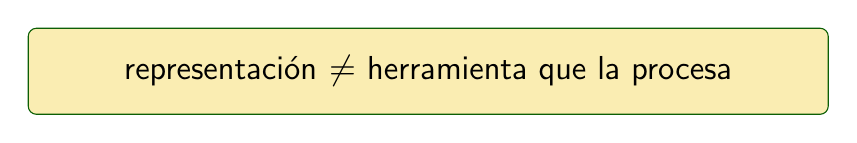
\begin{tikzpicture}
\node[idea, fill=pastelyellow, text width=.78\textwidth, inner sep=10pt, font=\large]
{representación \(\neq\) herramienta que la procesa};
\end{tikzpicture}
\end{center}

\vfill
\end{frame}

\begin{frame}{Trabajo con el cuadernillo}
\vfill

\begin{center}
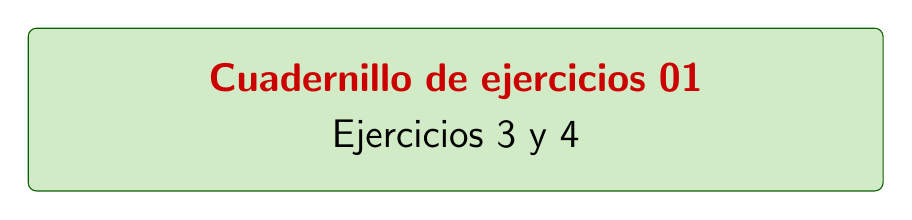
\begin{tikzpicture}
\node[
  idea,
  fill=pastelgreen,
  text width=.82\textwidth,
  inner sep=13pt,
  font=\Large
]
{\actividad{Cuadernillo de ejercicios 01}\\[2pt]
Ejercicios 3 y 4};
\end{tikzpicture}
\end{center}

\bigskip

\begin{itemize}
\item \textbf{Esencial --- Ejercicio 3:} relacionar herramientas y responsabilidades.
\item \textbf{Extensión --- Ejercicio 4:} completar el recorrido del código fuente a la memoria.
\end{itemize}

\vfill
\end{frame}

\begin{frame}{Compiladores e intérpretes}
\vfill

\begin{columns}[T,onlytextwidth]
\begin{column}{.48\textwidth}
\begin{block}{Compilador}
\small
Lee un programa en un lenguaje fuente y lo traduce a un programa equivalente en un lenguaje destino. También informa los errores que puede detectar durante la traducción.
\end{block}
\end{column}
\begin{column}{.48\textwidth}
\begin{block}{Intérprete}
\small
Ejecuta las operaciones especificadas por el programa fuente a partir de las entradas, sin producir como resultado principal un programa destino independiente.
\end{block}
\end{column}
\end{columns}

\vfill
\end{frame}

\begin{frame}{Dos modelos de procesamiento}
\vfill

\begin{center}
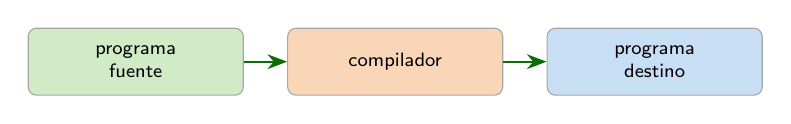
\begin{tikzpicture}[node distance=.55cm]
\node[mini, fill=pastelgreen, text width=2.45cm] (f) {programa\\fuente};
\node[mini, fill=pastelpeach, right=of f, text width=2.45cm] (c) {compilador};
\node[mini, fill=pastelblue, right=of c, text width=2.45cm] (d) {programa\\destino};
\draw[arrow] (f) -- (c);
\draw[arrow] (c) -- (d);
\end{tikzpicture}

\bigskip

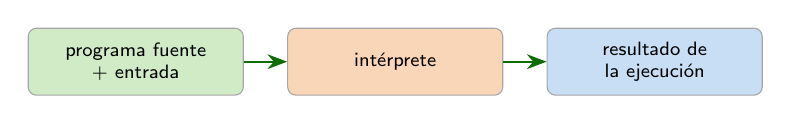
\begin{tikzpicture}[node distance=.55cm]
\node[mini, fill=pastelgreen, text width=2.45cm] (f2) {programa fuente\\+ entrada};
\node[mini, fill=pastelpeach, right=of f2, text width=2.45cm] (i) {intérprete};
\node[mini, fill=pastelblue, right=of i, text width=2.45cm] (s) {resultado de\\la ejecución};
\draw[arrow] (f2) -- (i);
\draw[arrow] (i) -- (s);
\end{tikzpicture}
\end{center}

\bigskip

\begin{center}
\term{Traducir un programa no es lo mismo que ejecutar sus operaciones.}
\end{center}

\vfill
\end{frame}

\begin{frame}{Los modelos pueden combinarse}
\vfill

\begin{center}
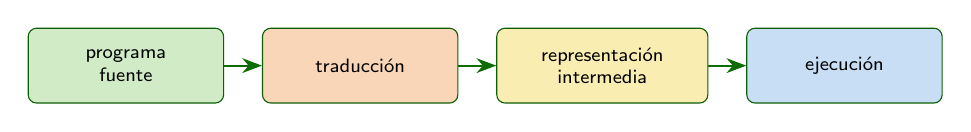
\begin{tikzpicture}[node distance=.48cm]
\node[paso, fill=pastelgreen, text width=2.2cm] (a) {programa\\fuente};
\node[paso, fill=pastelpeach, right=of a, text width=2.2cm] (b) {traducción};
\node[paso, fill=pastelyellow, right=of b, text width=2.4cm] (c) {representación\\intermedia};
\node[paso, fill=pastelblue, right=of c, text width=2.2cm] (d) {ejecución};
\draw[arrow] (a) -- (b);
\draw[arrow] (b) -- (c);
\draw[arrow] (c) -- (d);
\end{tikzpicture}
\end{center}

\bigskip

\begin{block}{Lo importante para el repaso}
Los modelos básicos ayudan a distinguir responsabilidades. Un sistema real puede combinar traducción y ejecución sin que ambas acciones se vuelvan equivalentes.
\end{block}

\vfill
\end{frame}

\begin{frame}{Trabajo con el cuadernillo}
\vfill

\begin{center}
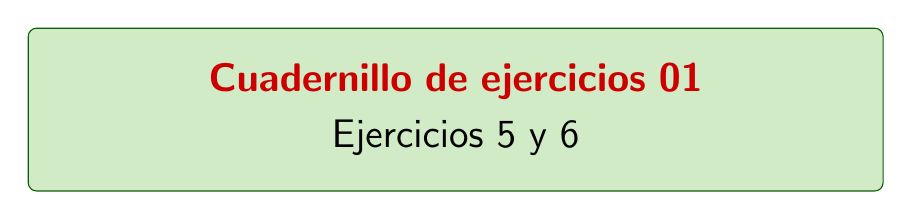
\begin{tikzpicture}
\node[
  idea,
  fill=pastelgreen,
  text width=.82\textwidth,
  inner sep=13pt,
  font=\Large
]
{\actividad{Cuadernillo de ejercicios 01}\\[2pt]
Ejercicios 5 y 6};
\end{tikzpicture}
\end{center}

\bigskip

\begin{itemize}
\item \textbf{Esencial --- Ejercicio 5:} comparar compilador e intérprete.
\item \textbf{Extensión --- Ejercicio 6:} identificar el modelo descrito en cada situación.
\end{itemize}

\vfill
\end{frame}

\begin{frame}{El compilador del curso}
\vfill

\begin{center}
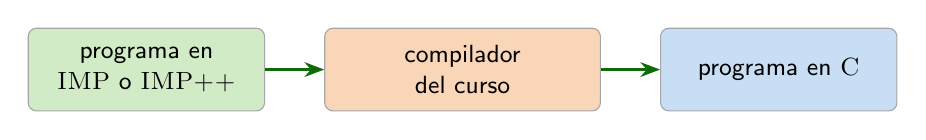
\begin{tikzpicture}[node distance=.75cm]
\node[bloque, fill=pastelgreen, text width=2.65cm] (a) {programa en\\\textsc{IMP} o \textsc{IMP++}};
\node[bloque, fill=pastelpeach, right=of a, text width=3.15cm] (b) {compilador\\del curso};
\node[bloque, fill=pastelblue, right=of b, text width=2.65cm] (c) {programa en \textsc{C}};
\draw[arrow] (a) -- (b);
\draw[arrow] (b) -- (c);
\end{tikzpicture}
\end{center}

\bigskip

\begin{block}{Un producto, dos momentos}
En notas y clase construiremos el compilador del \textsc{IMP} base. En las prácticas extenderemos ese mismo producto para \textsc{IMP++}; ambas versiones producirán \textsc{C}.
\end{block}

\vfill
\end{frame}

\begin{frame}{Cuatro ideas que recorrerán el curso}
\vfill

\begin{center}
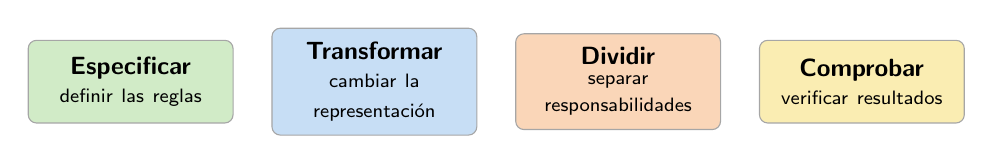
\begin{tikzpicture}[node distance=.48cm]
\node[bloque, fill=pastelgreen, text width=2.25cm] (a) {\textbf{Especificar}\\[-1pt]\scriptsize definir las reglas};
\node[bloque, fill=pastelblue, right=of a, text width=2.25cm] (b) {\textbf{Transformar}\\[-1pt]\scriptsize cambiar la representación};
\node[bloque, fill=pastelpeach, right=of b, text width=2.25cm] (c) {\textbf{Dividir}\\[-1pt]\scriptsize separar\\[-1pt]\scriptsize responsabilidades};
\node[bloque, fill=pastelyellow, right=of c, text width=2.25cm] (d) {\textbf{Comprobar}\\[-1pt]\scriptsize verificar resultados};
\end{tikzpicture}
\end{center}

\bigskip

\begin{center}
\small Las cuatro aparecen en un mismo producto acumulativo, aunque se trabajarán progresivamente.
\end{center}

\vfill
\end{frame}

\begin{frame}{Trabajo con el cuadernillo}
\vfill

\begin{center}
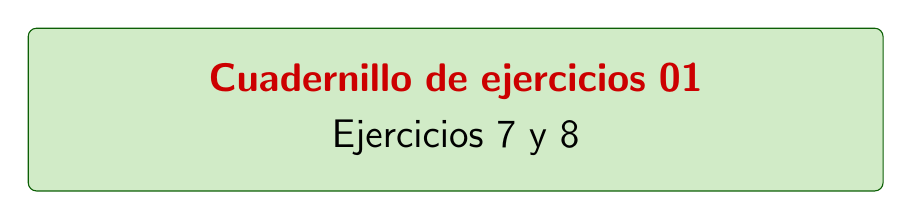
\begin{tikzpicture}
\node[
  idea,
  fill=pastelgreen,
  text width=.82\textwidth,
  inner sep=13pt,
  font=\Large
]
{\actividad{Cuadernillo de ejercicios 01}\\[2pt]
Ejercicios 7 y 8};
\end{tikzpicture}
\end{center}

\bigskip

\begin{itemize}
\item \textbf{Extensión --- Ejercicio 7:} relacionar decisiones con las cuatro ideas.
\item \textbf{Esencial --- Ejercicio 8:} distinguir el lenguaje base, su extensión y el destino \textsc{C}.
\end{itemize}

\vfill
\end{frame}

\begin{frame}{Confusiones que debemos evitar}
\vfill

\begin{center}
\small
\renewcommand{\arraystretch}{1.22}
\begin{tabular}{|L{.39\textwidth}|L{.46\textwidth}|}
\hline
\textbf{Confusión} & \textbf{Corrección} \tabularnewline
\hline
Compilador e intérprete hacen lo mismo. & Uno traduce; el otro ejecuta las operaciones indicadas. \tabularnewline
\hline
El cargador forma el ejecutable. & El ligador forma el ejecutable; el cargador lo coloca en memoria. \tabularnewline
\hline
Lenguaje ensamblador y ensamblador son lo mismo. & Uno es una representación; el otro es una herramienta. \tabularnewline
\hline
La programación de sistemas se limita a sistemas operativos. & Incluye diversas herramientas que apoyan la operación y ejecución de programas. \tabularnewline
\hline
\end{tabular}
\end{center}

\vfill
\end{frame}

\begin{frame}{Trabajo con el cuadernillo}
\vfill

\begin{center}
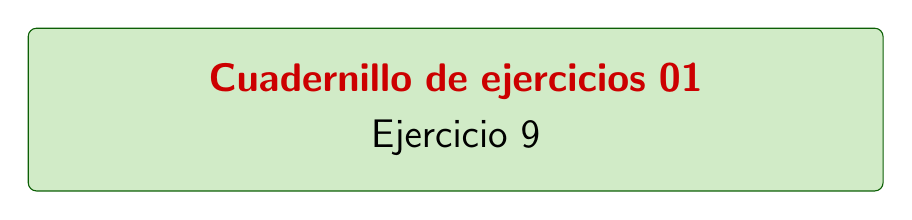
\begin{tikzpicture}
\node[
  idea,
  fill=pastelgreen,
  text width=.82\textwidth,
  inner sep=13pt,
  font=\Large
]
{\actividad{Cuadernillo de ejercicios 01}\\[2pt]
Ejercicio 9};
\end{tikzpicture}
\end{center}

\bigskip

\begin{itemize}
\item \textbf{Extensión --- Ejercicio 9:} detectar la parte incorrecta de cada afirmación.
\item Reescribir cada idea de forma adecuada.
\end{itemize}

\vfill
\end{frame}

\begin{frame}{Conclusión}
\vfill

\begin{center}
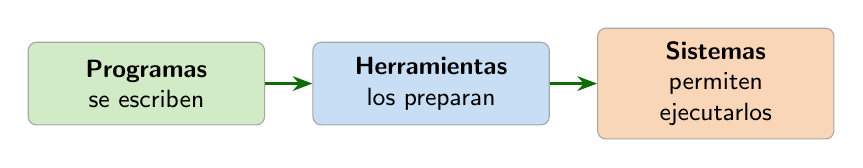
\begin{tikzpicture}[node distance=.6cm]
\node[bloque, fill=pastelgreen, text width=2.65cm] (a) {\textbf{Programas}\\se escriben};
\node[bloque, fill=pastelblue, right=of a, text width=2.65cm] (b) {\textbf{Herramientas}\\los preparan};
\node[bloque, fill=pastelpeach, right=of b, text width=2.65cm] (c) {\textbf{Sistemas}\\permiten ejecutarlos};
\draw[arrow] (a) -- (b);
\draw[arrow] (b) -- (c);
\end{tikzpicture}
\end{center}

\bigskip

\begin{block}{Idea de cierre}
La programación de sistemas estudia y construye software que conecta lenguajes, programas y recursos de cómputo. El compilador será nuestro caso para observar esa relación de forma acumulativa.
\end{block}

\vfill
\end{frame}

\begin{frame}{Referencias}
\vfill

\scriptsize
\begin{enumerate}
\item Soto Romero, M. y Reyes Cabello, A. L. (2026). \textit{Programación de Sistemas. Nota de clase 01: Panorama de la programación de sistemas}. Colegio de Ciencia y Tecnología, UACM.
\item Soto Romero, M. y Reyes Cabello, A. L. (2026). \textit{Programación de Sistemas. Cuadernillo de ejercicios 01: Panorama de la programación de sistemas}. Colegio de Ciencia y Tecnología, UACM.
\item Beck, L. L. (1996). \textit{System Software: An Introduction to Systems Programming} (3.\textsuperscript{a} ed.). Addison-Wesley. ISBN: 978-0-201-42300-6.
\item Bala, K., Bracy, A., Sirer, E. y Weatherspoon, H. (2025). \textit{Compilation---Assemblers, Linkers, \& Loaders}. CS 3410 [diapositivas].
\item Aho, A. V., Lam, M. S., Sethi, R. y Ullman, J. D. (2006). \textit{Compilers: Principles, Techniques, and Tools} (2.\textsuperscript{a} ed.). Pearson/Addison-Wesley.
\item Vilar Torres, J. M. (2010). \textit{Estructura de los compiladores e intérpretes}. Universitat Jaume I.
\end{enumerate}

\vfill
\end{frame}

\end{document}
